% !TEX root = main.tex
\section{EXPERIMENTS}
\label{sec: experiments}
%In this section, we compare the three types of inference methods discussed before, namely the classical approach of conjugate dual inference (CDI), AVI and ACP. 
We compare the performance of different inference methods on both synthetic and real-world datasets. The synthetic datasets are described in section \ref{sec: experiment setup}. We use them as the ground-truth is known.  
%We compare the performance of each inference method under two different settings, namely scarce vs sufficient training data (See table \ref{tab: syndata}).
We investigate how the characteristics of different approaches vary with respect to the amount of training data in section~\ref{sec: experiment inference}-\ref{sec: experiment density estimation}. 
The real-world dataset is described  in section \ref{sec:topicmodels} and is used to illustrate one of the practical uses of the inference methods in topic modeling.  
Our experiments show that the proposed ACP method outperforms other variational approaches in most cases.
%We perform empirical studies on synthetic datasets in sections~\ref{sec: experiment inference} --~\ref{sec: experiment density estimation}. Results on real data are reported in section~\ref{sec:topicmodels}.
%Section \ref{sec: experiment setup} describes the experiment setup, including dataset and implementation details. Section \ref{sec: experiment inference} compares different inference strategies in terms of inference accuracy. In Section \ref{sec: parameter estimation}, we visualize the learned And in section \ref{sec: experiment density estimation}, we compare the density estimation results of AVI and ACP under different scenarios.

\subsection{Synthetic Datasets}
\label{sec: experiment setup}
\begin{table}[t]
\caption{\small Parameters for synthetic datasets of \emph{patterned} weights}
\label{tab: syndata}
\centering
%\begin{minipage}{0.8\columnwidth}
%\centering
{\small
\resizebox{\columnwidth}{!}{%
\begin{tabular}{lccccc}
\toprule
 Dataset & $D$ & $K$ & $\mu_k$  & $N_{test}$ & Sparsity  \\
\midrule
 \pattern & 64 & 8 & 0.125 & 1000 & 89.0\%\\
 \textsc{multi-mnist} & 784 & 10 & 0.2 & 5000 & 80.3\% \\
\bottomrule
\end{tabular}%
}
}
\end{table}
\begin{table}[t]
\caption{\small Parameters for synthetic datasets of \emph{random} weights (\sparse)}
\label{tab: syndata2}
\centering
{\small
\begin{tabular}{cccccccc}
\toprule
\small
 size & $\alpha_{\btheta}$ & $\beta_{\btheta}$ & $\alpha_{\bmu}$ & $\beta_{\bmu}$ & $s$ & $N_{test}$ & Sparsity  \\
\midrule
\multirow{3}{*}{\parbox{1.2cm}{$D=50$ $K\!=\!100$}} & 1 &	5 & 1 & 10 & 0.95 & 1000 & 94.2\% \\
  & 2 & 5 & 2 & 5 & 0.95 & 1000 & 71.8\% \\
  & 2 & 5 & 2 & 5 & 0.9 & 1000 & 51.4\% \\
\hline
\multirow{3}{*}{\parbox{1.2cm}{$D\!=\!500$ $K\!=\!500$}}& 1 & 5 & 1 & 20 & 0.995 & 2000 & 98.4\% \\
& 1 & 20 & 1 & 20	& 0.95 & 2000 & 95.3\%\\
 & 1 & 10 & 1 & 10 & 0.95 & 2000 & 73.6\% \\
%\midrule
\hline
\parbox{1.2cm}{$D\!=\!500$ $K\! =\!100$} & 1 & 5 & 1 & 5 & 0.95 & 5000 & 89.2\% \\
\bottomrule
\end{tabular}
}
%\end{minipage}
\vspace{-1em}
\end{table}

For reproducibility, we detail the learning and optimization hyperparameters in the Supplementary Materials. 
\paragraph{Data with Patterned Weights} We created this type of synthetic datasets with the following recipe:
\begin{itemize}
\setlength\itemsep{0em}
    \item Select the parameters $\mu_k$ of the prior distributions $p(z_k=1) = \mu_k$, $k = 1 \cdots K$.
    \item Select the generative model parameter $\btheta \in \mathbb{R}^{D\times K}$ and the ``leak'' probability $\btheta_0 \in \mathbb{R}^{D}$. $\btheta$ and $\btheta_0$ needs to be non-negative.
    \item Sample $N$ latent variables $\bz^{(n)}$, $n=1, \cdots, N$ from the prior distribution $p(\bz)$.
    \item Sample $N$ observed data points $\bx^{(n)}$ from the conditional probability $p(\bx^{(n)}|\bz^{(n)})$.
\end{itemize}
where $K$ is the number of latent variables and $D$ is the number of observed variables. The two types of datasets are described below.

We generated two datasets: \pattern and \textsc{multi-mnist}. The configurations of $D$, $K$ and $\mu_k$ are specified in Table \ref{tab: syndata}.
The model parameters $\btheta$ and $\btheta_0$ are reshaped from the patterns depicted in Fig. \ref{fig: sub toy pattern} (\pattern) and \ref{fig: mnistpattern} (\textsc{multi-mnist}). 
%Each pattern is a $8 \times 8$ matrix and reshaped to a $64$-dimensional vector representing $\btheta_k \in \mathcal{R}^{64}$, 
Each pattern is reshaped to a $D$-dimensional vector representing $\btheta_k \in \mathcal{R}^{D}$, 
where the white pixels in the $k$th pattern indicates the corresponding parameters $\theta_{ik}$ to be 0.
And the last pattern refers to the pattern of ``leak'' probability. 
The values of non-zero $\theta_{ik}$ (\ie, black pixels) are $-\log(1-0.8)$ which means $p(x_i=1|z_k=1)=0.8$. 
%We then compute $\theta_{ik}$ as $\theta_{ik} = -\log(1-p_{ik})$.
Fig. \ref{fig: patternsample} and \ref{fig: mnistsample} show some data points sampled from the two datasets. Each data point is a combination of their parameter patterns with missing parts. 
We use $N_{test}$ data points for validation and another $N_{test}$ for testing. The values of $N_{test}$ are reported in Table \ref{tab: syndata}.
%We split $N_{test}$ data points into validation and test set.\todo{you never actually say how many is used for test and $N_{test}$ is the number of test points or total number of data points?}


\begin{figure}[t!]
    \centering
    \begin{minipage}[b]{0.4\columnwidth}
        \centering
        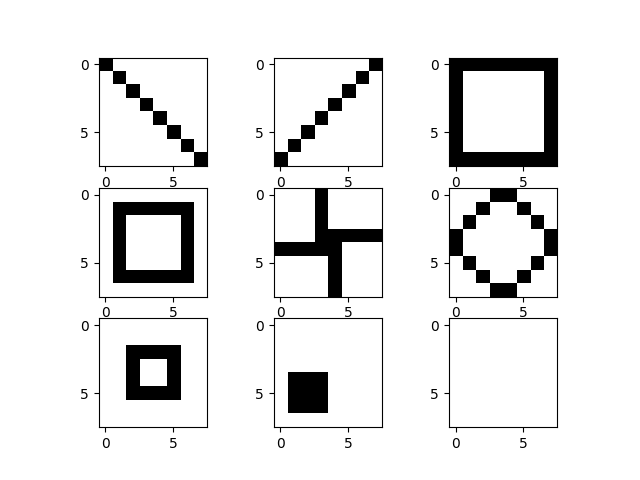
\includegraphics[width=1\linewidth]{pattern.png}
        \subcaption{}\label{fig: sub toy pattern}
    \end{minipage}%
    \begin{minipage}[b]{0.4\columnwidth}
        \centering
        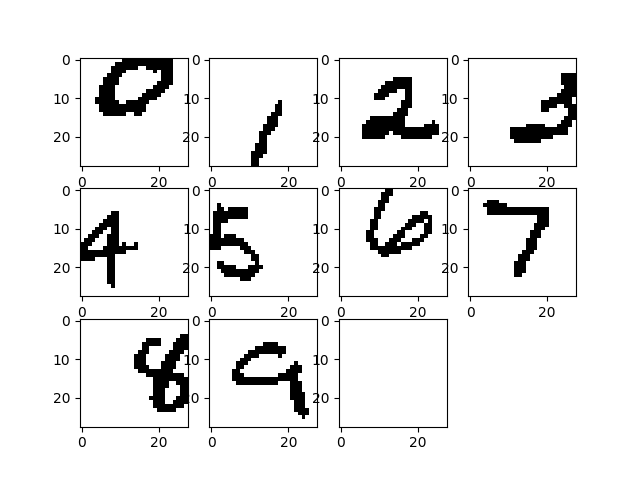
\includegraphics[width=1\linewidth]{multimnistpattern.png}
       \subcaption{}\label{fig: mnistpattern}
    \end{minipage}
    \begin{minipage}[b]{0.4\columnwidth}
        \centering
        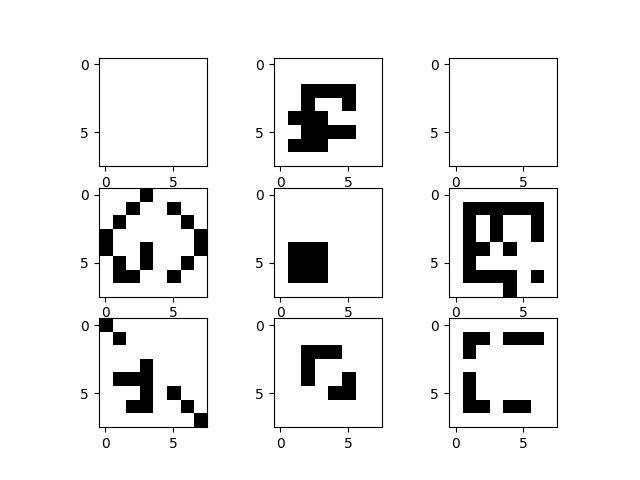
\includegraphics[width=1\linewidth]{figs/toy_data.png}
        \subcaption{}\label{fig: patternsample}
    \end{minipage}%
    \begin{minipage}[b]{0.4\columnwidth}
        \centering
        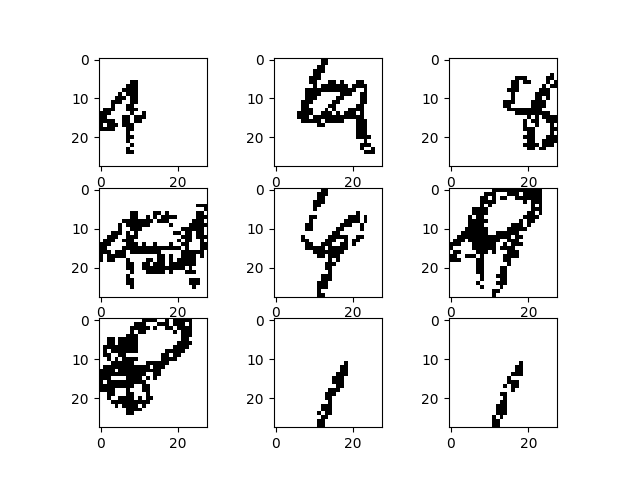
\includegraphics[width=1\linewidth]{multimnistsamples.png}
       \subcaption{}\label{fig: mnistsample}
    \end{minipage}
    \caption{\small (a) and (b). The patterns of the parameters $\btheta$ for the \pattern and \textsc{multi-mnist} datasets, respectively. (c) and (d). Several observed $\bx$, sampled from the \pattern and \textsc{multi-mnist} datasets.}
    \label{fig: pattern data}
    \vskip -1em
\end{figure}

\paragraph{Data with Random Weights}
We also built a synthetic datasets with random sampled weights, namely \sparse. 
Concretely, $\btheta$, $\btheta_0$ and $\bmu$ are sampled from distributions $\textsc{Beta}(\alpha_{\btheta}, \beta_{\btheta})$ and $\textsc{Beta}(\alpha_{\bmu}, \beta_{\bmu})$. Moreover, the sparsity of the dataset is controlled by constraining the sparsity degree $s$ to be $0<s<1$, which can be viewed as the probability of removing the connection between $z_k$ and $x_i$ by setting $\theta_{ik}=0$, to enforce the sparse connections between latent and observed variables. The random removal of those connections can create orphaned variables without any connections. Thus, we randomly add connections to the latent and observed variables which do not have any connection. We describe the configurations of \sparse\  in Table~\ref{tab: syndata2}. 
%We distinguish two types of datasets: a \textsc{small} version and \textsc{large} version where $D$ and $K$ are both small or both large.

The \textsc{Sparsity} is defined as the percentage of negative observations in the dataset $\textsc{Sparsity} = \frac{1}{ND}\sum_{n=1}^N \sum_{i=1}^D \mathbb{I}(x^{(n)}_i=0)$
%\begin{equation}
%\textsc{Sparsity} = %\frac{1}{ND}\sum_{n=1}^N %\sum_{i=1}^D %\mathbb{I}(x^{(n)}_i=0)
%\end{equation}
where lower \textsc{Sparsity} value indicates denser dataset. %where $N_{test} = 1000$ for the \textsc{small} models and $N_{test} = 2000$ for the \textsc{large} models.


 
%The anonymized links to download datasets used and codes for running the experiments are \url{https://sites.google.com/view/acp-data-code}.

\begin{figure*}[t!]
    \centering
    \begin{minipage}[b]{0.9\columnwidth}
{\tiny
%Inference performance on  dataset\\
\resizebox{0.9\columnwidth}{!}{%
\begin{tabular}{|c|c|ccc|}

\hline
$N_{train}$ & Method & NELBO & F1 & EM \\
\hline 
\multirow{2}{*}{1000} & AVI & \textbf{14.0} & \textbf{94.5} & \textbf{91.0} \\
                      & ACP & 14.4 & 94.3 & 90.4 \\
\hline
\multirow{2}{*}{100} & AVI & 18.4 & 86.6 & 76.8 \\
                     & ACP & \textbf{17.4} & \textbf{87.1} & \textbf{81.1} \\
\hline
\multirow{2}{*}{20} & AVI & 37.2 & 49.2 & 47.6 \\
                     & ACP & \textbf{22.2} & \textbf{76.1} & \textbf{64.0} \\
\hline
\multirow{3}{*}{--} 
& SVI & 22.6 & 62.5 & 43.0 \\
& LB-CDI & 22.4 & 63.6 & 45.4 \\
& UB-CDI & 96.6 & 24.6 & 39.0 \\


\hline
\end{tabular}%
}
}
\subcaption{}\label{tab: toy data experiment}
     \end{minipage}
\begin{minipage}[b]{0.8\columnwidth}
\centering
    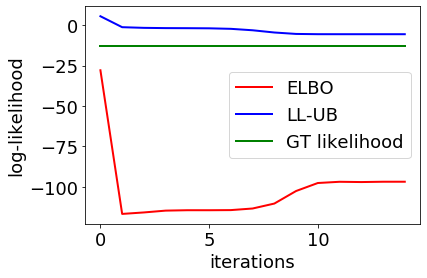
\includegraphics[width=0.7\linewidth]{CDI.png}
    \subcaption{}
    \label{fig: CDI learning curve}
\end{minipage}
\vspace{-0.3cm}
\caption{\small Inference results on \pattern. (a).  NELBO: negative ELBO (lower is better).  Higher F1 and EM are better. (b). The learning curve of UB-CDI. It shows that tighter variational bound does not imply better approximate posterior.}
\vskip -1em
\end{figure*}
\subsection{Inference}
\label{sec: experiment inference}
%Herein, we compare the CDI, AVI and ACP on their abilities of accurately approximating the posterior distribution. 
Herein, we compare ACP with baselines on their abilities of accurately approximating the posterior distribution.
We fix the generative model with its ground truth parameters, and evaluate the accuracy of inference by computing the ELBO with respect to different approximate posterior distributions on the \emph{held-out} data. Since the generative model is fixed, the ELBO is maximized when $\pqx= p(\bz|\bx; \btheta)$. Hence higher ELBO indicates better inference performance. Moreover, we  compare the ground truth $\bz^{(n)}$ and $\hat{\bz}^{(n)} \sim q(\bz|\bx^{(n)}; \bphi), n = 1, \cdots, N$ using macro F1 and Exact Match (EM) scores as inference accuracy.


We analyzed two types of CDI, namely UB-CDI and LB-CDI as CDI with variational Upper-Bound and Lower-Bound respectively.
The parameters in CDI are optimized following the optimization strategy in~\citep{jaakkola1999variational, vsingliar2006noisy}, where we find the tightest likelihood upper-bound (or lower-bound) using fix-point optimization and use it to compute posterior (eq.~(\ref{eqTightBound})). %ASVI is optimized by maximizing the lower-bound of ELBO. 
Similarly, SVI is trained to maximize the lower-bound of the ELBO.

For AVI and ACP,  the variational parameters $\bphi$ are optimized to maximize the ELBO. 
We report the results of learned $\bphi$ under different amount of training data. For non-amortized methods SVI and CDI, we optimize the variational parameter on samples from held-out set directly.
%\subsubsection{Evaluate Inference Strategies}
%We evaluate our ACP model and the baselines on \pattern dataset and report the performance on the held-out set with different amount of training data. 
 %We use $1000$ data points in the held-out set for evaluation.



Fig.~\ref{tab: toy data experiment} shows the experiment results, where $N_{train}$ indicates the number of training data. 
We observe that with a sufficient amount of training data ($N_{train}=1000$), AVI achieves slightly better performance due to its high flexibility to approximate the posterior. Yet when we have only limited amount of training data, ACP gains huge advantages over AVI. %As we reduce the number of training data, the gap between ACP and AVI becomes wider.

%We observe that ACP shows huge advantage over AVI when we do not have sufficient training data because of its special formulation for posterior distribution. 
%When we have sufficient training data, although AVI achieves better performance due to its higher capacity of representing more accurate approximate posterior, the difference is not significant and can be ignored.
 %We find ACP could be useful in applications where the training data is hard to acquire.


%Surprisingly, CDI achieves very poor performance. 
We observed that UB-CDI achieves very poor performance. 
The learning curve of UB-CDI is depicted in Fig. \ref{fig: CDI learning curve}, where LL-UB indicates the Log-Likelihood Upper-Bound:
\begin{align*}
\log \tp(\bx|\bphi)  =& \log \sum_{\bz} \prod_{i:x_i=1} \tp(x_i=1|\bz, \bphi) \cdot\\
&\prod_{j:x_j=0}p(x_j=0|\bz)p(\bz).
\end{align*}
In the first $10$ rounds of fix-point optimization, LL-UB becomes tighter as we optimize more iterations and then converges. However, with a tighter upper-bound, the ELBO first drops quickly, and then improves \emph{only slightly} during optimization. The final ELBO after convergence is much worse, even comparing to  the initial point. This observation indicates that a tighter likelihood upper-bound is not necessarily equivalent to a better approximate posterior. Thus we will not compare to UB-CDI in the rest of our experiments.

Although LB-CDI is also optimized to obtain the tightest bound, its performance is much better than UB-CDI. The reason is that LB-CDI optimizes the lower-bound of ELBO. As it optimizes the lower-bound, the ELBO is pushed up. However the performance of LB-CDI is still much worse than amortized methods when training data is sufficient. Hence, optimizing the ELBO directly is very helpful comparing to optimizing its approximation. The low performance of SVI confirms this observation. 

%Note that while SVI performance does not rely on the number of training samples, ACP (and AVI) can improve rapidly with the increasing number of parameters.  
Note that while SVI performance does not rely on the number of training samples, ACP (and AVI) can improve rapidly with the increasing number of training data.  
In particular, since ground-truth parameters are generally not known and need to be learned from data, we anticipate ACP and AVI have more advantages in the learning setting, which we describe below.
\begin{figure*}[t]
    \centering
    \begin{subfigure}[t]{0.2\textwidth}
        \centering
        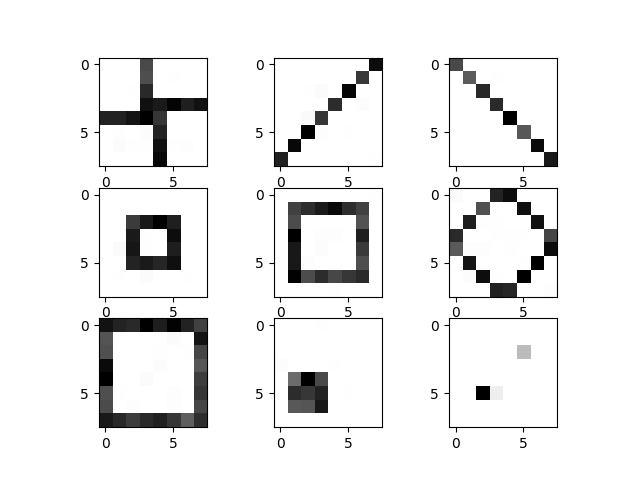
\includegraphics[width=1.0\linewidth]{AVI_1000.png}
        \caption{AVI, $N_{train}=1000$}
        \label{fig: avi1000}
    \end{subfigure}%
    ~
    \begin{subfigure}[t]{0.2\textwidth}
        \centering
        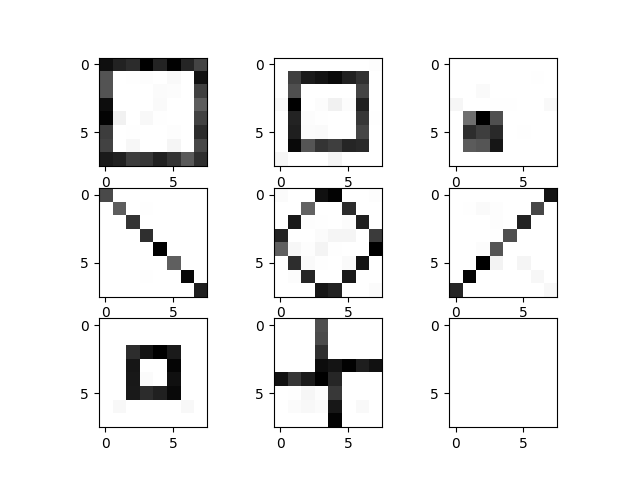
\includegraphics[width=1.0\linewidth]{ACP_1000.png}
        \caption{ACP, $N_{train}=1000$}
        \label{fig: ACP1000}
    \end{subfigure}%
    ~
    \begin{subfigure}[t]{0.2\textwidth}
        \centering
        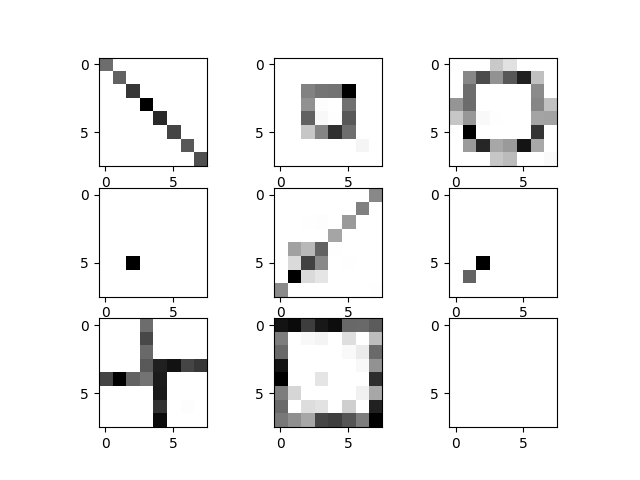
\includegraphics[width=1.0\linewidth]{AVI_200.png}
        \caption{AVI, $N_{train}=200$}
        \label{fig: avi200}
    \end{subfigure}%
    ~
    \begin{subfigure}[t]{0.2\textwidth}
        \centering
        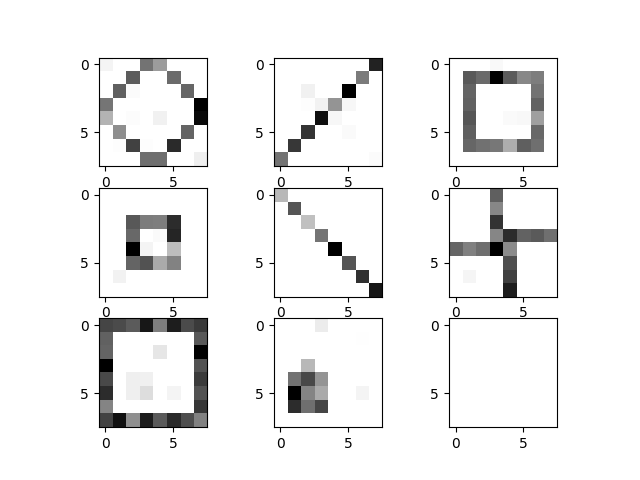
\includegraphics[width=1.0\linewidth]{ACP_200.png}
        \caption{ACP, $N_{train}=200$}
        \label{fig: ACP200}
        \vskip -1em
    \end{subfigure}
    \vspace{-0.3cm}
\caption{\small The recovered parameters of \pattern after training with $1000$ and $200$ data points using AVI and ACP.}
\label{fig: parameter estimation}
\end{figure*}

\subsection{Parameter Estimation}
\label{sec: parameter estimation}
To further analyze the properties of ACP, we jointly train the generative and inference models on \pattern and \textsc{multi-mnist} dataset. The goal is to recover the patterns of $\btheta$ in a fully unsupervised way, and compare the performance of ACP over the baselines with different amount of training data.
%how the amount of training data affects the performance of AVI and ACP.
 

Fig. \ref{fig: parameter estimation} shows the  results for AVI and ACP on \pattern \footnote{Due to the low performance of SVI and LB-CDI, their results are moved to the Supplementary Materials.}.
 From Fig. \ref{fig: avi1000} and \ref{fig: ACP1000}, we observe that both AVI and ACP recover all the patterns and achieve similar performance. When reducing the amount of training data to $200$ (Fig. \ref{fig: avi200} and \ref{fig: ACP200}), we observe that ACP still reconstructs all the patterns with slightly worse performance. In contrast, the performance of AVI degrades more severely. Specifically, two patterns out of the eight are not recovered (\ie the middle left and middle right patterns in Fig. \ref{fig: avi200}). Additionally, some patterns are merged (\ie the upper right and middle patterns in Fig. \ref{fig: avi200}). This result indicates that model dependent posterior form is helpful in structured inference for learning useful latent representations, especially when we have small amount of training data. Similarly, we perform experiments on \textsc{multi-mnist} dataset. The results are reported in the Supplementary Materials.  %This result indicates that the model dependent posterior form is helpful in structured inference and learning useful latent representations, especially when we have small amount of training data.

%While when we reduce the amount of training data to $200$, 

%When we have sufficient training data, ACP-dp and AVI achieves on par performance by recovering all the patterns succesfully, yet ACP-idp has worse result. 
%However, when we only have limited number of training data (ie, $N=200$), the performance of AVI degrades severely. Two out of eight latent variables do not learn any useful representation. ACP-dp achieves the best performance by observing all the correct patterns. 



%in Fig. \ref{fig: parameter estimation multimnist}. Since \textsc{multi-mnist} has more training data and larger dimensionality, it is hard to perform LB-CDI on it. Thus we only compared ACP with AVI and SVI. The result of SVI is shown in Supplementary Material. \todo{todo: put SVI to supplementary material}



\begin{figure*}[t]
    \centering
    \begin{subfigure}[t]{0.3\textwidth}
        \centering
        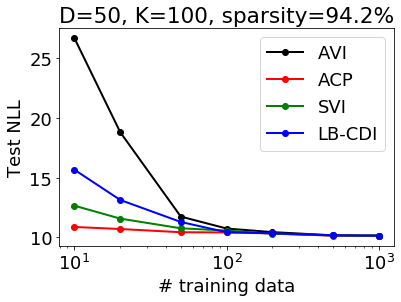
\includegraphics[height=1.2in]{100_50.png}
        \caption{}
        \label{fig: 6a}
    \end{subfigure}%
    ~ 
    \begin{subfigure}[t]{0.3\textwidth}
        \centering
        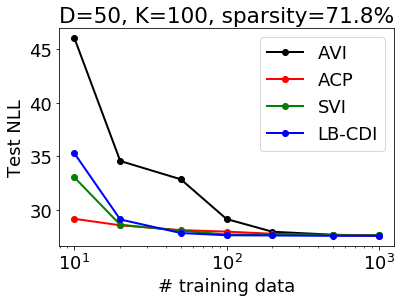
\includegraphics[height=1.2in]{100_50_dense.png}
        \caption{}
    \end{subfigure}%
    ~
    \begin{subfigure}[t]{0.3\textwidth}
        \centering
        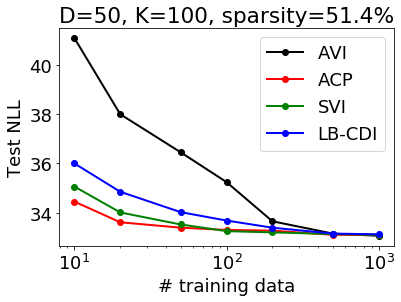
\includegraphics[height=1.2in]{100_50_denser.png}
        \caption{}
        \label{fig: 6c}
    \end{subfigure}
    ~
    \begin{subfigure}[t]{0.3\textwidth}
        \centering
        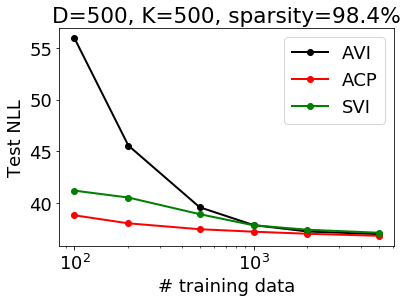
\includegraphics[height=1.2in]{500_500.png}
        \caption{}
    \end{subfigure}%
    ~ 
    \begin{subfigure}[t]{0.3\textwidth}
        \centering
        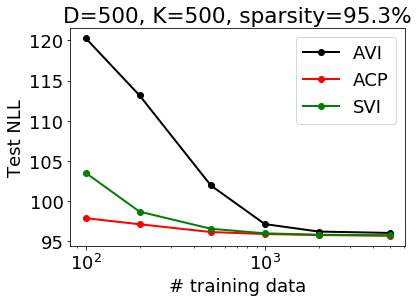
\includegraphics[height=1.2in]{500_500_dense.png}
        \caption{}
    \end{subfigure}
    ~
    \begin{subfigure}[t]{0.3\textwidth}
        \centering
        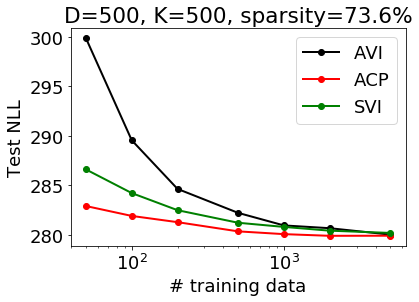
\includegraphics[height=1.2in]{500_500_denser.png}
        \caption{}
    \end{subfigure}
     \vspace{-0.2cm}
    \caption{\small Comparison of AVI and ACP in \textsc{noisy-or} under different model structure and different data sparsity.}
    \vspace{0.2cm}
\label{fig: compare avi ACP sparsity}
\vskip -1em
\end{figure*}



%\subsection{Generalization with small and sparse training data}
\subsection{Generative Modeling with Synthetic Datasets}
\label{sec: experiment density estimation}

While the previous sections focus on comparing methods on inference accuracy and parameter recovery, this section focuses on generative modeling and compares methods in the metric of negative ELBO on held-out set. 
%In this part, we investigate in detail how  ACP leads to better generalization comparing to AVI, and conducts better density estimation comparing to SVI and LB-CDI. 
According to eq.~(\ref{eq:factorizedposterior}), sparse data requires less parameter $\bpsi$ to be approximated. Thus, in addition to varying the amount of training data,  we also control the sparsity of the dataset and evaluate how it would affect the generative modeling. %We evaluate the performance using the negative ELBO on held-out set. 
%Note that AVI and ACP uses exactly the same training objective and same generative model. The only difference between this two methods is how they approximate the posterior distribution. So this is a fair comparison. 
We use \sparse datasets described in Table~\ref{tab: syndata} for these studies.



Fig.~\ref{fig: compare avi ACP sparsity} shows the experiment results with different amount of training data in various degrees of sparsity. ACP consistently outperforms competing methods. It performs on-par or slightly better than SVI, AVI and LB-CDI when using a large amount of data but performs noticeably better when using a small amount of data. 
%As we increase the size of training set, the performance of AVI improves quickly and achieves the similar performance to ACP. 
%In \citep{jaakkola1999variational}, the authors suggest that less sparse data results in worse approximation as the variational bound is applied to an increased number of positive observations. 
%In~\citep{jaakkola1999variational}, the authors suggest that more approximation on positive evidence nodes results in worse likelihood upper-bound.
Intuitively, denser data will result in worse approximation as the variational bound is applied to an increased number of positive observations.
%In Fig. \ref{fig: compare avi ACP sparsity}, we observe that both ACP and AVI are affected by this phenomenon. 
%However, ACP is less affected than AVI, specially when the amount of data is limited. In particular, the relative improvement of ACP over AVI is bigger when the data is sparser. 
However, in Fig.~\ref{fig: compare avi ACP sparsity}, we observe that ACP is not affected much by this phenomenon. An explanation is that ACP is not optimized to achieve the tightest variational bound, yet to improve the overall performance with respect to the ELBO. 

\begin{table}[t]
\caption{\small Generative modeling on \sparse, where $D=500$, $K=100$, $sparsity=89.2\%$}
\label{tab: densityestimation}
\centering
\resizebox{0.8\columnwidth}{!}{
\begin{tabular}{|c|c|c|c|c|}
\hline
$N_{train}$    & AVI   & SVI   & LB-CDI & ACP            \\ \hline
40k & 150.7 & 156.3 & -      & \textbf{149.5} \\ \hline
20k & 151.0 & 156.5 & -      & \textbf{149.8} \\ \hline
10k & 156.0 & 156.9 & -      & \textbf{150.3} \\ \hline
5k  & 157.6 & 157.4 & -      & \textbf{151.2} \\ \hline
1k  & 159.2 & 158.0 & 158.8  & \textbf{157.2} \\ \hline
\end{tabular}
}
\end{table}

Table \ref{tab: densityestimation} shows the modeling results on \sparse with $500$ observed and $100$ latent variables. Here we did not experiment LB-CDI with large training size (greater than 5k) due to the computational complexity. From Table \ref{tab: densityestimation}, we can observe that our ACP achieves on-par or slightly better performance comparing with AVI when we have sufficient training data, while SVI is significantly worse than both amortized approaches. When we have limited training data, the performance of AVI degrades faster than ACP. The large variance of AVI leads to the worst performance when the training set is limited. Our ACP method outperforms AVI and SVI with both sufficient and limited training data.

%we  observe that for both small and large model, the relative likelihood gaps (the y-axis in figures) become smaller as we decrease the sparsity of data. For instance, when we have $10$ training points, the relative likelihood gap in Fig. \ref{fig: 6a} is approximately $15$ out of $12$, while reduces to $15$ out of $35$ in Fig. \ref{fig: 6c}. The observation indicates that although ACP outperforms AVI when we have limited training data under all sparsity, ACP will obtain more performance gain over AVI on sparse data.  
%However, although in ACP we also only approximate the positive conditional probability, the performance of ACP seems \emph{unaffected} by the sparsity of the dataset. The reason is that we optimize the inference model to maximize the ELBO instead of finding the tightest bound. Hence, adding more positive observations would indeed affect the tightness of the variational bound, but not necessarily the accuracy of approximate posterior in ACP. 

\begin{table*}[h!]
\caption{\small Top 10 words inferred on NeurIPS Titles dataset for top 4 topics with 5241 and 2000 training data.}
\vspace{-0.3cm}
    \label{tab: topicmodelfull}
    \centering
     \tiny
    \resizebox{0.88\textwidth}{!}{
    \begin{tabular}{|c|c|c|c||c|c|c|c|}
    %\hline
         %\multicolumn{8}{|c|}{$N_{train}=5241$}\\
    \hline
         \multicolumn{4}{|c||}{$N_{train}=5241$, ACP (PMI = \textbf{2.78}) } &  \multicolumn{4}{|c|}{$N_{train}=5241$, AVI (PMI = 2.49)  }  \\
     \hline
  Topic 1   &  Topic 2    &  Topic 3   & Topic 4    & Topic 1    & Topic 2    & Topic 3    & Topic 4 \\
     \hline 
classification &bayesian &  sparse  & application    &process & process  &  multi   & sparse  \\
application &base&analysis&classification &inference&inference&bayesian& regression\\
via &optimization&deep& process&gaussian&bayesian&probabilistic& gaussian\\
method &adaptive&datum& linear &markov&analysis&information&via \\
process  &method&method&stochastic &datum&gaussian&inference& estimation\\
multi &function&estimation&analysis  &mixture&datum&dynamic&inference \\
bayesian &object&multi& multi&analysis&mixture&approach& analysis\\
kernel &estimation&feature& datum&bayesian&variational&function& linear\\
feature &information&convex&time &variational&approach&application&process \\
image &datum&probabilistic& via&dynamic&probabilistic&process& optimization\\
                \hline
          PMI : \textbf{3.82}  &   PMI : 3.22&  PMI :  3.18  &   PMI : \textbf{3.16}  &   PMI : 3.74 &   PMI : \textbf{3.73}&  PMI : \textbf{3.69} & PMI : 2.98\\
                 \hline
\hline
%\multicolumn{8}{|c|}{$N_{train}=2000$} \\
%\hline
         \multicolumn{4}{|c||}{$N_{train}=2000$, ACP (PMI = \textbf{2.75})} &  \multicolumn{4}{|c|}{$N_{train}=2000$, AVI  (PMI = 2.55)}  \\
     \hline
  Topic 1   &  Topic 2    &  Topic 3   & Topic 4    & Topic 1    & Topic 2    & Topic 3    & Topic 4 \\
     \hline 
image  &kernel &method   &inference  &  base   &  optimization    &  feature   & process          \\
feature &base&estimation&bayesian& adaptive &sparse   & function   &  gaussian\\
   optimization  &image&sparse&process&   process& recognition  & base   &  via\\
     application   &process&non&classification&  kernel  & classification  &datum    &datum  \\
        recognition  &dynamic&stochastic&kernel&   method & method  &information    & inference \\
          fast &estimation&optimization&multi&  linear  & base  &   adaptive &  optimization\\
         clustering  &classification&application&analysis&   datum  & adaptive  &  reinforcement  &time  \\
          via  &deep&gradient&linear&  system & linear  & search   & recognition \\
          representation &optimal&multi&fast&   sample  &  function &gaussian    &base  \\
           reinforcement &sample&fast&application&  dynamic  &  regression &   bound &  latent\\
               
                \hline
      PMI : \textbf{3.47}   &   PMI : \textbf{3.40}  &  PMI :  \textbf{3.20}   &   PMI :  \textbf{3.19}  &   PMI : 3.09 &   PMI : 3.00 &  PMI : 2.95 & PMI : 2.91\\
                 \hline
    \end{tabular}}
    \vskip -1em
\end{table*}

\subsection{Topic Models}
\label{sec:topicmodels}

We compare AVI and ACP on topic modeling.
%In fact, as existing latent factor models \citep{blei2003latent, ranganath2015deep}, once learned, the latent representations can be used to identify document topics. 
We use the titles of all the Neural Information Processing Systems (NeurIPS) papers from  1987 to 2016~\citep{nipsdata}.  Each observed data point $\bx^{(n)}$ is a $D$-dimensional binary vector representing a paper's title, where $D$ is the size of the vocabulary. The value of $x_i^{(n)}$, $i=1, \cdots, D$ indicates the presence/absence of word $w_i$ in the $n$-th title. 
After word lemmatization, removing stop words, the $5$ most common words and the words with less than $5$ occurrences in the whole corpus, we obtain a dataset with $7241$ data points and $1216$ unique words. The average length of the paper title is $4.49$ after pre-processing. 
We use $1000$ data points for validation, $1000$ for testing, and the remaining ones for training. We model the data with $K=20$ latent variables. 

Each latent variable $z_k$ is interpreted as a topic capturing a distribution of words. To further show the semantic coherence of words in each topic, we report the  point-wise mutual information (PMI), which has been shown to be highly correlated with human judgment in assessing word relatedness~\citep{newman2009external}, between word pairs of each topic. To do so we use the whole English $\tt WIKIPEDIA$ corpus, that consists of approximately 4 millions of documents and 2 billions of words. The PMI between two words $w_i$ and $w_j$ is given by $\text{PMI}(w_i,w_j)=\log \frac{p(w_i,w_j)}{p(w_i) p(w_j)}$,
%\begin{align}
%    \text{PMI}(w_i,w_j)=\log \frac{p(w_i,w_j)}{p(w_i) p(w_j)}
%\end{align}
 where  $p(w_i)$  is the probability that word $w_i$ occurs in  $\tt WIKIPEDIA$, and $p(w_i,w_{j})$ is the probability that words $w_i$ and $w_{j}$ co-occur in a 5-word window in any $\tt WIKIPEDIA$ document. Higher PMIs indicate higher semantic coherence.
 %, the more the words are semantically coherent.


Table~\ref{tab: topicmodelfull} reports the results by each model. We report the best 4 topics in terms of PMI and visualize their top-10 words. The words $w_i$ for topic $z_k$ are selected with the highest parameters $\theta_{ik}$, which corresponds to the highest value $p(x_i=1|z_k)$.  We also report the average pairwise PMI between the top words within each topic, and the mean of the average pairwise PMI across all topics.
With more training data ($N_{train}=5241$), ACP and AVI achieve similar average PMI.  When $N_{train}$ is reduced to $2000$, all four selected topics in ACP have better average pairwise PMI scores than AVI. 
In Supplementary Materials, we report additional experimental results of document classification and latent representations of the learnt topics.
\iffalse
\begin{table*}[!ht]
\caption{Top 10 words inferred on NeurIPS Titles dataset for top 4 topics with \textbf{2000} training data.}
    \label{tab: topicmodel2000}
    \centering
    \resizebox{0.9\textwidth}{!}{
    \begin{tabular}{|c|c|c|c||c|c|c|c|}
    \hline
         \multicolumn{4}{|c||}{ACP (PMI = 2.75)} &  \multicolumn{4}{|c|}{AVI  (PMI = 2.55)}  \\
     \hline
  Topic 1   &  Topic 2    &  Topic 3   & Topic 4    & Topic 1    & Topic 2    & Topic 3    & Topic 4 \\
     \hline 
image  &kernel &method   &inference  &  base   &  optimization    &  feature   & process          \\
feature &base&estimation&bayesian& adaptive &sparse   & function   &  gaussian\\
   optimization  &image&sparse&process&   process& recognition  & base   &  via\\
     application   &process&non&classification&  kernel  & classification  &datum    &datum  \\
        recognition  &dynamic&stochastic&kernel&   method & method  &information    & inference \\
          fast &estimation&optimization&multi&  linear  & base  &   adaptive &  optimization\\
         clustering  &classification&application&analysis&   datum  & adaptive  &  reinforcement  &time  \\
          via  &deep&gradient&linear&  system & linear  & search   & recognition \\
          representation &optimal&multi&fast&   sample  &  function &gaussian    &base  \\
           reinforcement &sample&fast&application&  dynamic  &  regression &   bound &  latent\\
               
                \hline
      PMI : \textbf{3.47}   &   PMI : \textbf{3.40}  &  PMI :  \textbf{3.20}   &   PMI :  \textbf{3.19}  &   PMI : 3.09 &   PMI : 3.00 &  PMI : 2.95 & PMI : 2.91\\
                 \hline
    \end{tabular}}
\end{table*}
\fi





